\documentclass[11pt, oneside]{article}   	% use "amsart" instead of "article" for AMSLaTeX format
\usepackage{geometry}                		% See geometry.pdf to learn the layout options. There are lots.
\geometry{letterpaper}                   		% ... or a4paper or a5paper or ... 
%\geometry{landscape}                		% Activate for for rotated page geometry
%\usepackage[parfill]{parskip}    		% Activate to begin paragraphs with an empty line rather than an indent
\usepackage{graphicx}				% Use pdf, png, jpg, or eps� with pdflatex; use eps in DVI mode
								% TeX will automatically convert eps --> pdf in pdflatex		
\usepackage{amssymb}
\usepackage{amsmath}
\usepackage{parskip}
\usepackage{hyperref}

\title{Integration:  examples (part 2)}
%\author{The Author}
%\section{}
% \subsection*{R code}
\date{}							% Activate to display a given date or no date

\graphicspath{{/Users/telliott_admin/Dropbox/Tex/png/}}

\begin{document}
\maketitle
\Large
%\noindent

I came across an interesting problem in a chapter of Strogatz's \emph{The Joy Of x}.  He calls it the stovepipe problem.  We want to find the volume of the region formed from the intersection of two cylinders (of equal radius), that meet at right angles.

\begin{center} 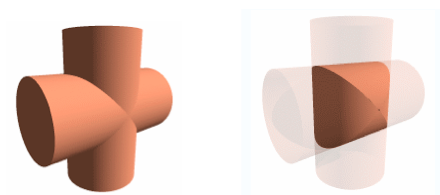
\includegraphics [scale=0.5] {stovepipe1.png} \end{center}

I really couldn't visualize it, but he told me that the horizontal cross sections of this solid are squares, and gave a picture.

\begin{center} 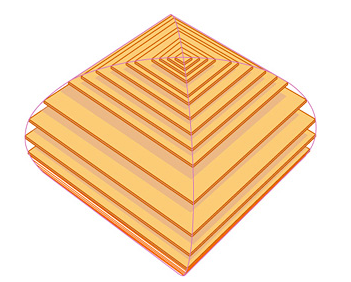
\includegraphics [scale=0.5] {stovepipe2.png} \end{center}

and it makes sense, if you imagine cutting through a potato with a cylindrical bore, then repeating at right angles.  At each level, the side is formed by cutting along the edge of the cylinder, hence the opposite sides are parallel.  And since the two cuts use the same cylinder, all $4$ sides at any particular height are equal, giving a square.

So our problem is to find the length of the side at each value of the height.  We deal with the upper half of the solid, for simplicity.  If you draw a sketch of the vertical cross-section, at each distance $h$ from the base of the solid, extending up, the remainder of the height down to the base is $R-h$, and the half-length of the side is $s/2 = \sqrt{R^2 - h^2}$.

The volume is obtained by adding up all these slices

\[ V = \int_0^R 2  \sqrt{R^2 -h^2} \ dh \]

Let's simplify the problem further (for the moment) by dealing with the case where $R=1$  We need the integral

\[ \int \sqrt{1-h^2} \ dh \]

I certainly didn't know that off the top of my head.

\section*{a new integral}

You know that the derivative of the inverse sine is:
\[ \frac{d}{dx} \sin^{-1} x  = \frac{1}{\sqrt{1-x^2}} \]

(The way we get this:  let $x = x/1 = \sin t$, then $t = \sin^{-1} x$ and $\sqrt{1-x^2} = \cos t$ and
\[ \frac{dx}{dt} = \cos t = \sqrt{1-x^2} \]
\[ \frac{dt}{dx} = \frac{1}{\cos t} = \frac{1}{\sqrt{1-x^2}} \] 

Now, how about 

\[ \int \sqrt{1-x^2} \ dx \]

It's the same term, but it's on top rather than in the denominator.  What happens if we multiply top and bottom by $\sqrt{1-x^2}$?

\[ = \int \frac{1-x^2}{\sqrt{1-x^2}} \ dx \]
\[ = \int \frac{1}{\sqrt{1-x^2}} \ dx + \int \frac{-x^2}{\sqrt{1-x^2}} \ dx \]

Is this progress?  Now we have an extra power of $x$ in the term on the right.  Since we know we can integrate the square root using one power of $x$, and taking the derivative of the remaining factor of $x$ will make it go away, it sounds like we should try integration by parts

\[ \int u \ dv = uv - \int v \ du \]

Let $x = u$, then $dx = du$.  And let $-x/\sqrt{1-x^2} \ dx$ = $dv$.  Then
\[ v = \sqrt{1-x^2} \]

So the integral of this part is

\[ \int \frac{-x^2}{\sqrt{1-x^2}} \ dx = x \sqrt{1-x^2} - \int  \sqrt{1-x^2} \ dx  \]

We still can't integrate the term on the right, but now, we have two of them!  Putting it all together:

\[  \int \sqrt{1-x^2} \ dx = \int \frac{1}{\sqrt{1-x^2}} \ dx + x \sqrt{1-x^2} - \int \sqrt{1-x^2} \ dx  \]

So

\[ 2 \int \sqrt{1-x^2} \ dx =   \sin^{-1} x + x \sqrt{1-x^2} \]
\[ \int \sqrt{1-x^2} \ dx = \frac{1}{2}  \sin^{-1} x + \frac{x}{2} \sqrt{1-x^2}  \]

One more thing.  Suppose we have

\[ \int \sqrt{a^2-x^2} \ dx \]

We can pull out the $a$ as follows

\[ = a \int \sqrt{1- (\frac{x}{a})^2} \ dx \]

Let $u = x/a$, then $a \ du = dx$ and we have

\[ = a^2 \int \sqrt{1- u^2} \ du \]

So the final answer is

\[ \int \sqrt{a^2-x^2} \ dx = \frac{a^2}{2} \ [ \ \sin^{-1} \frac{x}{a} + \frac{x}{a} \sqrt{1-(\frac{x}{a})^2} \ ] \]

which can be rearranged slightly

\[ = \frac{a^2}{2} \ \sin^{-1} \frac{x}{a} + \frac{x}{2} \sqrt{a^2-x^2}  \]

I'll leave it to you to figure out the whole volume for the general case with radius $R$.



\end{document}  